\documentclass[a4paper, 11pt]{article}
\usepackage{comment}
\usepackage{lipsum}
\usepackage{fullpage}
\usepackage[a4paper, total={7in, 10in}]{geometry}
\usepackage[fleqn]{amsmath}
\usepackage{amssymb,amsthm}
\newtheorem{theorem}{Theorem}
\newtheorem{corollary}{Corollary}
\usepackage{graphicx}
\usepackage{tikz}
\usetikzlibrary{arrows}
\usepackage{verbatim}
\usepackage{float}
\usepackage{xcolor}
\usepackage{mdframed}
\usepackage[shortlabels]{enumitem}
\usepackage{indentfirst}
\usepackage{hyperref}
\usepackage{listings}

\definecolor{pykw}{RGB}{0,0,180}
\definecolor{pystr}{RGB}{163,21,21}
\definecolor{pycom}{RGB}{0,128,0}
\definecolor{pybg}{RGB}{245,245,245}

\lstdefinestyle{pystyle}{
    language=Python,
    backgroundcolor=\color{pybg},
    basicstyle=\ttfamily\footnotesize,
    keywordstyle=\color{pykw}\bfseries,
    stringstyle=\color{pystr},
    commentstyle=\color{pycom}\itshape,
    numbers=left,
    numberstyle=\tiny\color{gray},
    numbersep=6pt,
    frame=single,
    framesep=4pt,
    breaklines=true,
    breakatwhitespace=true,
    showstringspaces=false,
    tabsize=4,
    captionpos=b
}
\lstset{style=pystyle}

\renewcommand{\thesubsection}{\thesection.\alph{subsection}}

\newenvironment{problem}[2][Problem]
    { \begin{mdframed}[backgroundcolor=gray!20] \textbf{#1 #2} \\}
    {  \end{mdframed}}

\newenvironment{solution}
    {\textit{Solution:}}
    {}

\renewcommand{\qed}{\quad\qedsymbol}

\begin{document}
\noindent
\large\textbf{Krishna Teja} \hfill \textbf{Assignment - \#3}   \\
Email: cs23btech11028@iith.ac.in \hfill ID: CS23BTECH11028 \\
\normalsize Course: AI3403 - Multi-Agent Systems \hfill Term: Autumn 2026\\
Instructor: Dr. Venkatraman Renganathan \hfill Due Date: $18^{th}$ September, 2026 \\
\noindent\rule{7in}{2.8pt}

%%%%%%%%%%%%%%%%%%%%%%%%%%%%%%%%%%%%%%%%%%%%%%%%%%%%%%%%%%%%%%%%%%%%%%%%%
% Problem 1
%%%%%%%%%%%%%%%%%%%%%%%%%%%%%%%%%%%%%%%%%%%%%%%%%%%%%%%%%%%%%%%%%%%%%%%%%
\begin{problem}{1}
$N = 20$. Generate a connected Erdos-Renyi graph, random initial positions in $\mathbb{R}^2$, and use formation control to display the name in capital letters, letter by letter. Record the sequence as an animation and give the public GitHub link.
\end{problem}
\begin{solution}

\textbf{GitHub link} (code + animation):\\
\url{https://github.com/krishnateja2314/cs23btech11028-mas-assignment3}

\medskip
My call name is Krishna, so the sequence is $K \to R \to I \to S \to H \to N \to A$.

\medskip
\textbf{Formation control update.} For each agent $i$, with neighbours $\mathcal{N}_i$ and desired offset $r_i \in \mathbb{R}^2$,
\begin{align*}
    u_i[k] = \sum_{j \in \mathcal{N}_i}\big[(p_j[k] - p_i[k]) - (r_j - r_i)\big], \qquad p_i[k+1] = p_i[k] + \Delta t \, u_i[k].
\end{align*}
For each letter the shape is drawn as a poly-line inside $[0,1]^2$ and I sample $N = 20$ points on it, distributed by stroke length. These $20$ points are the offsets $r_1, \ldots, r_{20}$. Parameters: $p = 0.3$, $\Delta t = 0.05$, $300$ iterations per letter, seed $= 7$.

\begin{figure}[H]
    \centering
    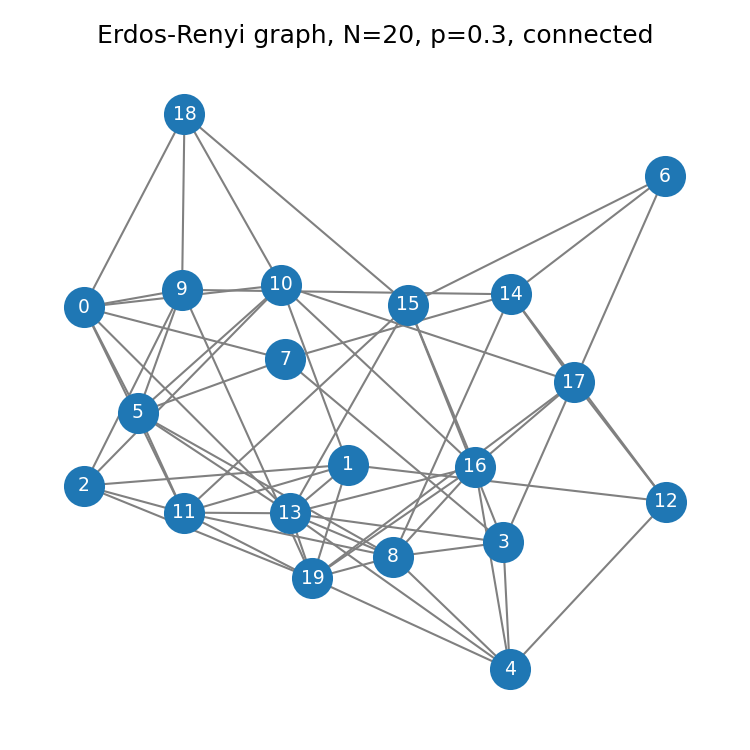
\includegraphics[scale=0.55]{../p1_formation/graph.png}
    \caption{Erdos-Renyi graph, $N=20$, $p=0.3$, connected.}
\end{figure}

\begin{figure}[H]
    \centering
    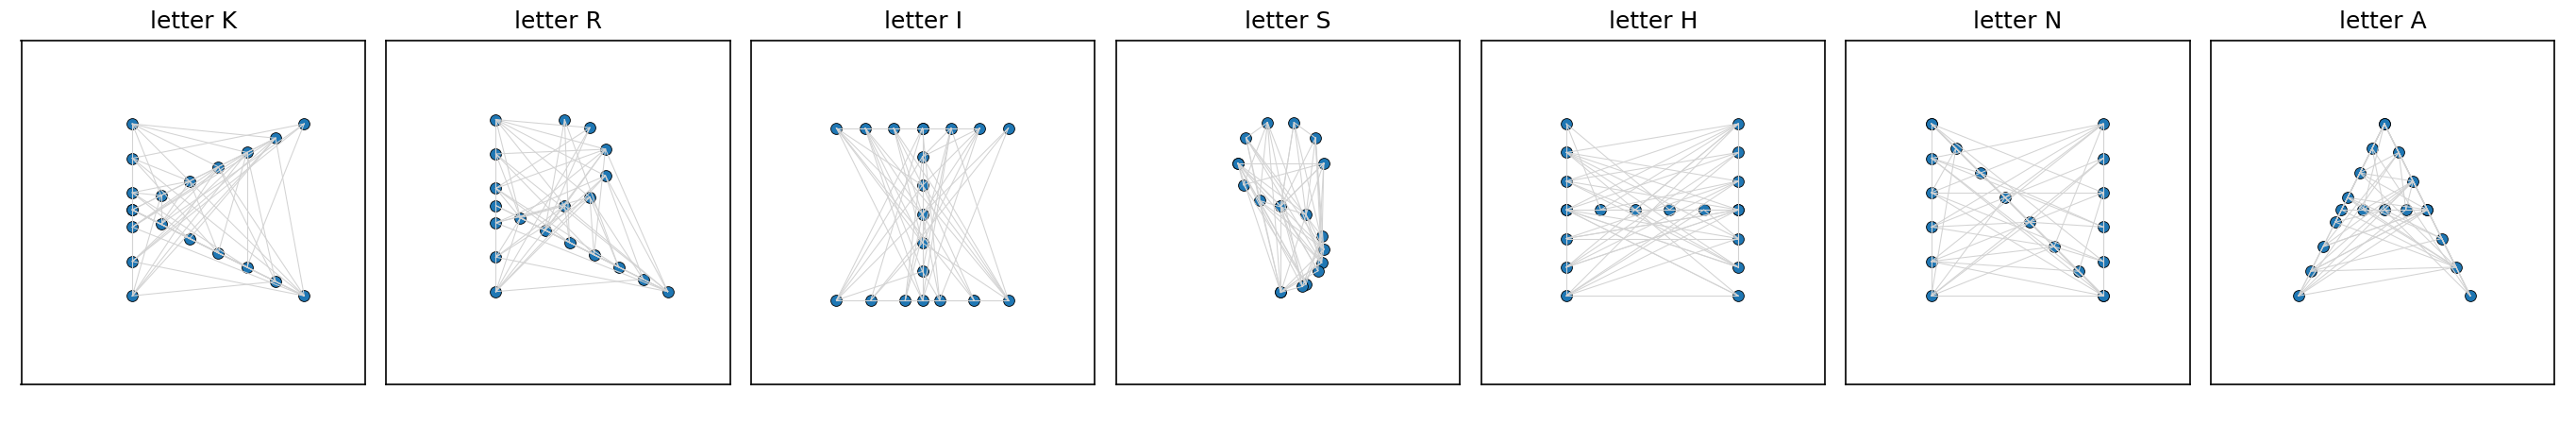
\includegraphics[width=\linewidth]{../p1_formation/letter_stills.png}
    \caption{Snapshots at the end of each letter phase: K R I S H N A.}
\end{figure}

\lstinputlisting[caption={\texttt{problem1\_formation.py}}]{../p1_formation/problem1_formation.py}

\end{solution}
\noindent\rule{7in}{2.8pt}

%%%%%%%%%%%%%%%%%%%%%%%%%%%%%%%%%%%%%%%%%%%%%%%%%%%%%%%%%%%%%%%%%%%%%%%%%
% Problem 2
%%%%%%%%%%%%%%%%%%%%%%%%%%%%%%%%%%%%%%%%%%%%%%%%%%%%%%%%%%%%%%%%%%%%%%%%%
\begin{problem}{2}
$N$ drones with sensors track an intruder $z(t) \in \mathbb{R}^3$ with dynamics $z(t+1) = z(t) + w$, $w \sim \mathcal{N}(0, \Sigma_w)$, and initial state $z(0) \sim \mathcal{N}(\bar z_0, \Sigma_0)$. Sensor $i$ is at $x_i \in \mathbb{R}^3$ and measures $y_i(t) = x_i - z(t) + v_i$ with $v_i \sim \mathcal{N}(0, \Sigma_v^{(i)})$, independent across $i$.
\begin{enumerate}[nosep]
    \item Formulate as consensus optimisation, specify each $f_i$.
    \item Estimate $\hat z(t)$ using DGD.
    \item Fix $N$, plot the graph, fix random parameters, simulate the true trajectory, plot $\hat z(t)$ vs $z(t)$ and report the error $e(t) = \hat z(t) - z(t)$.
\end{enumerate}
\end{problem}
\begin{solution}

\textbf{(1) Local objective $f_i$.} Given $z(t) = z$, $\;y_i(t) \mid z \sim \mathcal{N}(x_i - z,\, \Sigma_v^{(i)})$. The negative log likelihood (up to constants) is a weighted quadratic. The residual is $y_i(t) - (x_i - z) = y_i(t) - x_i + z$, so
\begin{align*}
    \boxed{\; f_i(z; t) \;=\; \tfrac{1}{2} \, \big\|\, y_i(t) - x_i + z \,\big\|^2_{(\Sigma_v^{(i)})^{-1}}, \qquad \nabla_z f_i(z; t) = (\Sigma_v^{(i)})^{-1}(y_i(t) - x_i + z). \;}
\end{align*}
The consensus form gives every drone a local copy $z_i \in \mathbb{R}^3$ and forces $z_i = z_j$ over the graph:
\begin{align*}
    \min_{z_1, \ldots, z_N} \frac{1}{N}\sum_{i=1}^{N} f_i(z_i; t) \qquad \text{s.t.} \quad z_i = z_j \;\;\forall (i,j) \in E.
\end{align*}

\textbf{(2) DGD update.} With mixing matrix $W$ (doubly stochastic, $W_{ij} = 0$ if $j \not\in \mathcal{N}_i$),
\begin{align*}
    z_i^{k+1} \;=\; \sum_{j=1}^{N} W_{ij} z_j^{k} - \alpha (\Sigma_v^{(i)})^{-1}(y_i(t) - x_i + z_i^k).
\end{align*}
I use Metropolis-Hastings weights $W_{ij} = 1/(1 + \max(\deg(i), \deg(j)))$ for edges and $W_{ii} = 1 - \sum_{j\ne i} W_{ij}$. At every $t$ I run $K_{\mathrm{inner}} = 120$ DGD steps with $\alpha = 0.5/L_{\mathrm{lip}}$ where $L_{\mathrm{lip}} = \sum_i 1/\sigma_i^2$.

\textbf{(3) Simulation.} $N = 8$, $p = 0.4$, $T_{\max} = 50$, $\bar z_0 = 0$, $\Sigma_0 = 4I$, $\Sigma_w = 0.05\, I$, $x_i \sim \mathcal{U}[-5, 5]^3$, $\Sigma_v^{(i)} = \sigma_i^2 I$ with $\sigma_i \sim \mathcal{U}[0.3, 0.8]$, seed $= 42$.

\begin{figure}[H]
    \centering
    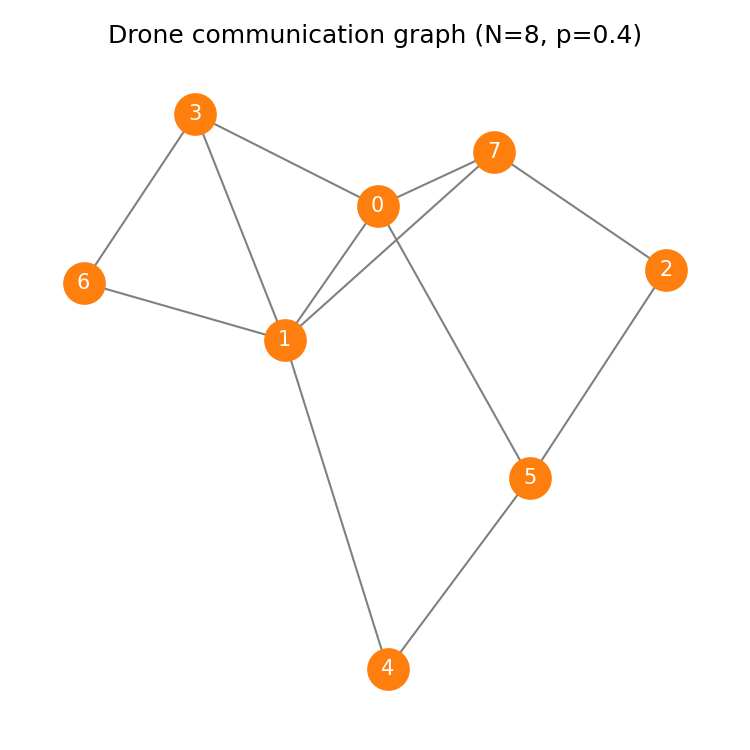
\includegraphics[scale=0.55]{../p2_dse/graph.png}
    \caption{Drone communication graph.}
\end{figure}

\begin{figure}[H]
    \centering
    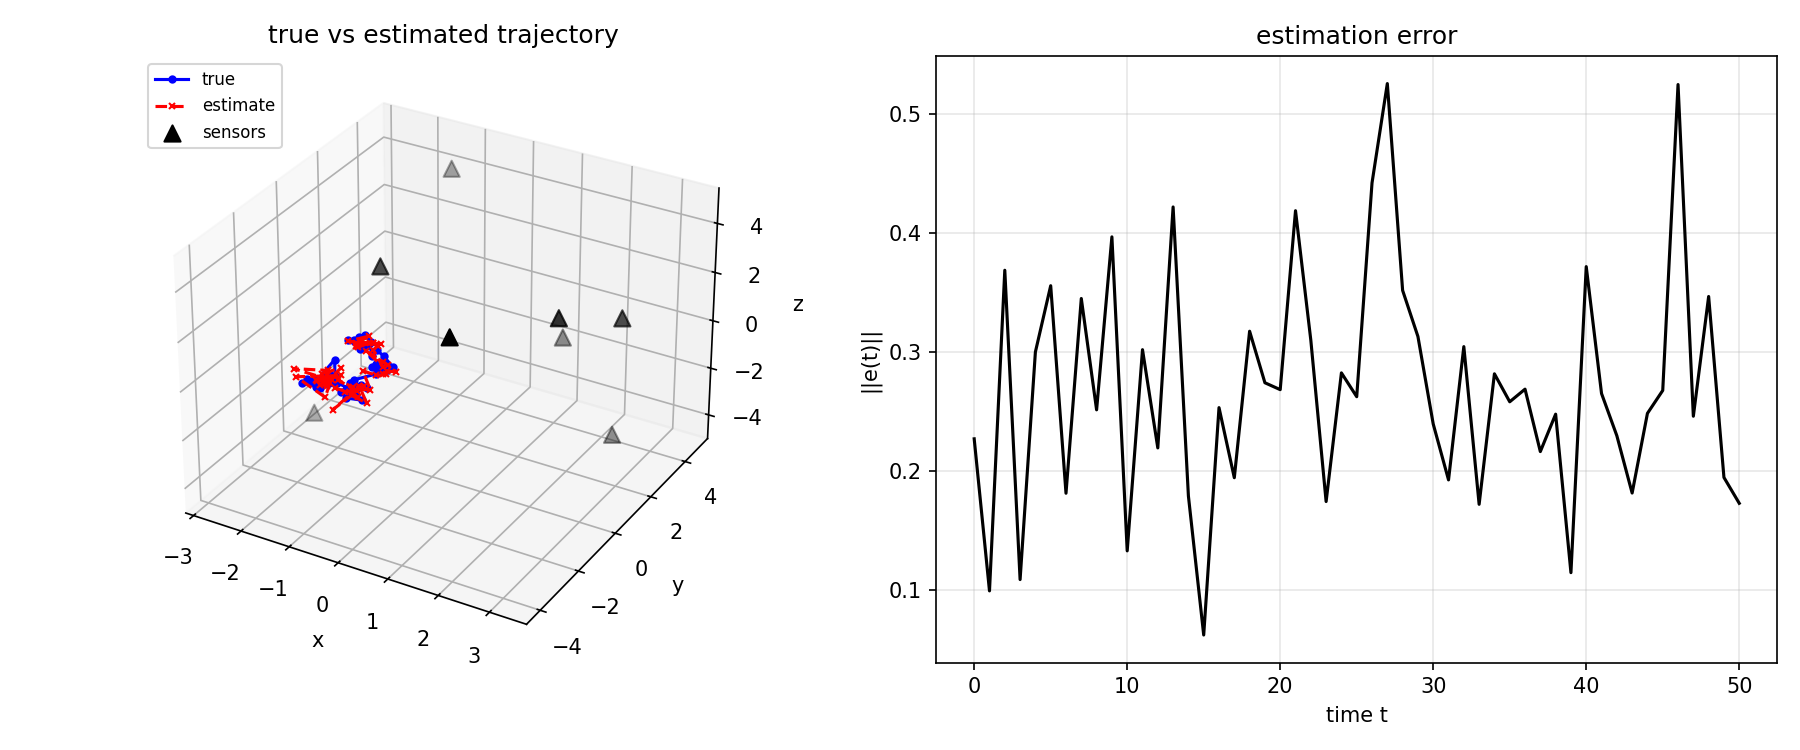
\includegraphics[width=\linewidth]{../p2_dse/estimate.png}
    \caption{Left: true (blue) vs estimated (red dashed) 3D trajectory with sensors (black triangles). Right: $\|e(t)\|_2$.}
\end{figure}

\begin{figure}[H]
    \centering
    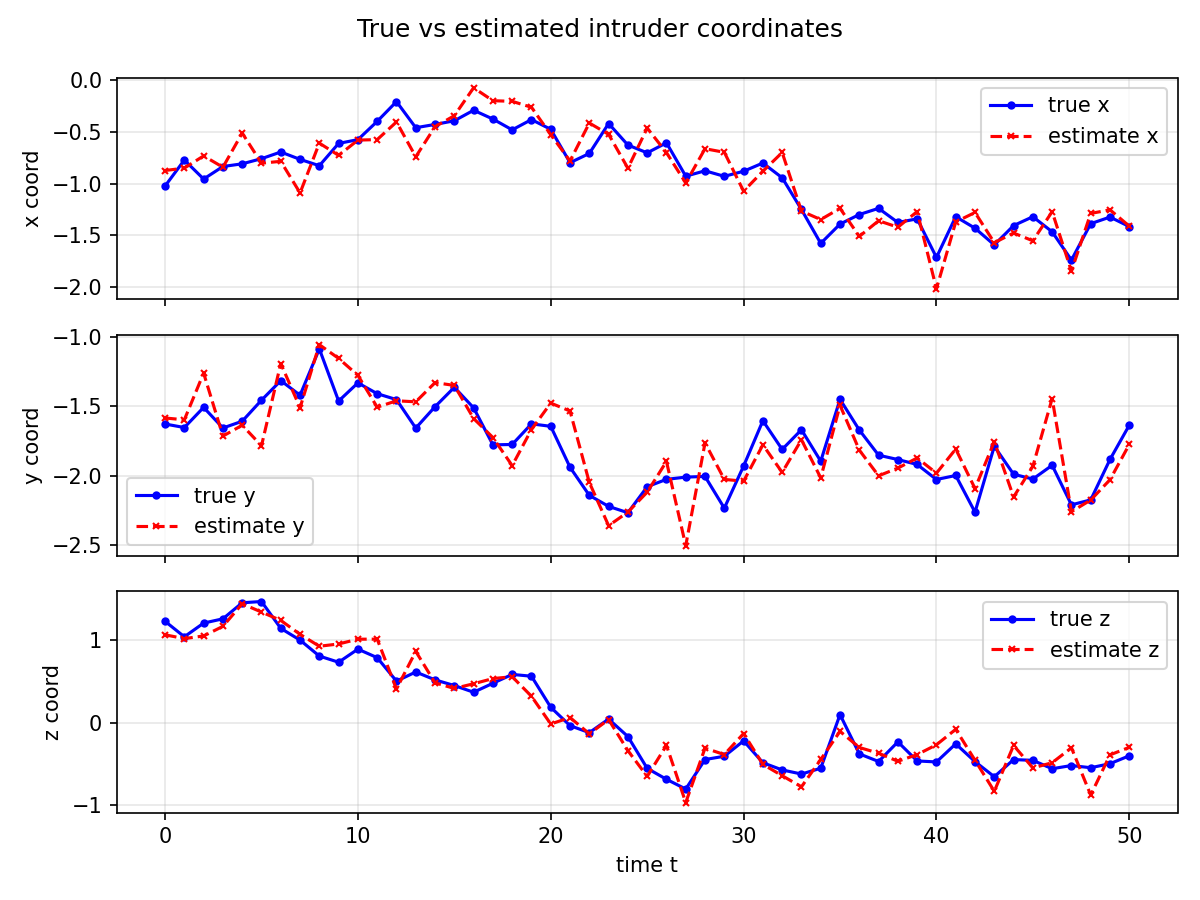
\includegraphics[width=0.85\linewidth]{../p2_dse/coord_trace.png}
    \caption{Per coordinate trace: true vs estimated.}
\end{figure}

Mean $\|e(t)\| \approx 0.27$, final $\|e(T)\| \approx 0.17$.

\lstinputlisting[caption={\texttt{problem2\_dse.py}}]{../p2_dse/problem2_dse.py}

\end{solution}
\noindent\rule{7in}{2.8pt}

%%%%%%%%%%%%%%%%%%%%%%%%%%%%%%%%%%%%%%%%%%%%%%%%%%%%%%%%%%%%%%%%%%%%%%%%%
% Problem 3
%%%%%%%%%%%%%%%%%%%%%%%%%%%%%%%%%%%%%%%%%%%%%%%%%%%%%%%%%%%%%%%%%%%%%%%%%
\begin{problem}{3}
$N$ agents on a connected undirected graph, $M > N$ tasks, cost matrix $C \in \mathbb{R}^{N \times M}_{>0}$, capacities $b_i \in \mathbb{Z}_{\geq 0}$ with $\sum_i b_i = M$, every task assigned exactly once.
\begin{enumerate}[nosep]
    \item Formulate as an optimisation problem, give ADMM updates for every agent. Do the convex relaxation of the binary LP.
    \item Fix $N, M$, generate connected ER graph, random capacities summing to $M$, positive cost matrix. Plot graph and allocation. Vary $C$ and comment.
\end{enumerate}
\end{problem}
\begin{solution}

\textbf{(1a) Binary linear program.} Let $x_{ij} \in \{0, 1\}$ be $1$ iff agent $i$ does task $j$:
\begin{align*}
    \min_{x} \sum_{i,j} C_{ij} x_{ij} \qquad \text{s.t.} \quad \sum_i x_{ij} = 1 \;\; \forall j, \quad \sum_j x_{ij} = b_i \;\; \forall i, \quad x_{ij} \in \{0, 1\}.
\end{align*}
This is an integer program, NP-hard in general.

\textbf{(1b) LP relaxation.} Replace $x_{ij} \in \{0,1\}$ by $0 \le x_{ij} \le 1$.

\textbf{(1c) Consensus ADMM.} Every agent $i$ holds a local copy $X^{(i)} \in \mathbb{R}^{N \times M}$ and a scaled dual $U^{(i)}$; there is one shared $Z$:
\begin{align*}
    \min \sum_i f_i(X^{(i)}) \qquad \text{s.t.} \quad X^{(i)} = Z, \qquad f_i(X) = \langle C_{i,:}, X_{i,:}\rangle + I_{\{0 \le X \le 1\}} + I_{\{\sum_j X_{i,j} = b_i\}},
\end{align*}
and the task-cover $\sum_i Z_{i,j} = 1$ is put on $Z$ as $g(Z)$.

\textbf{Scaled form ADMM updates for every agent $i$.} With penalty $\rho > 0$:
\begin{align*}
    X^{(i),k+1} &= \arg\min_X f_i(X) + \tfrac{\rho}{2}\|X - Z^k + U^{(i),k}\|_F^2, \\
    Z^{k+1}_{i,:} &= \tfrac{1}{|\mathcal{N}_i \cup \{i\}|} \sum_{j \in \mathcal{N}_i \cup \{i\}} (X^{(j),k+1}_{i,:} + U^{(j),k}_{i,:}), \quad \text{then project column sums to } 1, \\
    U^{(i),k+1} &= U^{(i),k} + (X^{(i),k+1} - Z^{k+1}).
\end{align*}

\textbf{Closed form of the $X$-update.} $f_i$ is separable over rows. For row $i$ set the unconstrained minimiser $r^{\star} = Z^k_{i,:} - U^{(i),k}_{i,:} - C_{i,:}/\rho$ and project onto the capped simplex $\{r : \sum_j r_j = b_i,\, 0 \le r_j \le 1\}$ (bisection). For every other row, clip $Z^k_{r,:} - U^{(i),k}_{r,:}$ to $[0, 1]$.

\textbf{Rounding.} The ADMM output may be fractional. I round it via linear sum assignment on the expanded matrix where agent $i$ is duplicated $b_i$ times (Hungarian on an $M \times M$ cost matrix, then collapse duplicates). The resulting matrix has row sums $b_i$ and column sums $1$ by construction.

\textbf{(2) Simulation.} $N = 5$, $M = 12$, $p = 0.5$, seed $= 3$, $\rho = 1$, $400$ iterations. Random positive composition of $M$ gives $b = [1, 1, 1, 4, 5]$. Three cost matrices are drawn from $\mathcal{U}(0.1, 10)$.

\begin{figure}[H]
    \centering
    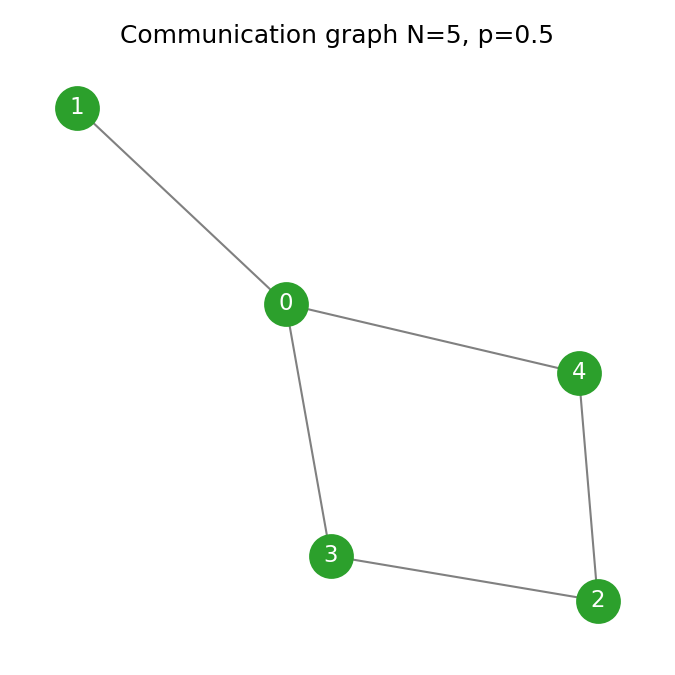
\includegraphics[scale=0.55]{../p3_admm_task/graph.png}
    \caption{Communication graph, $N=5$, $p=0.5$.}
\end{figure}

\begin{figure}[H]
    \centering
    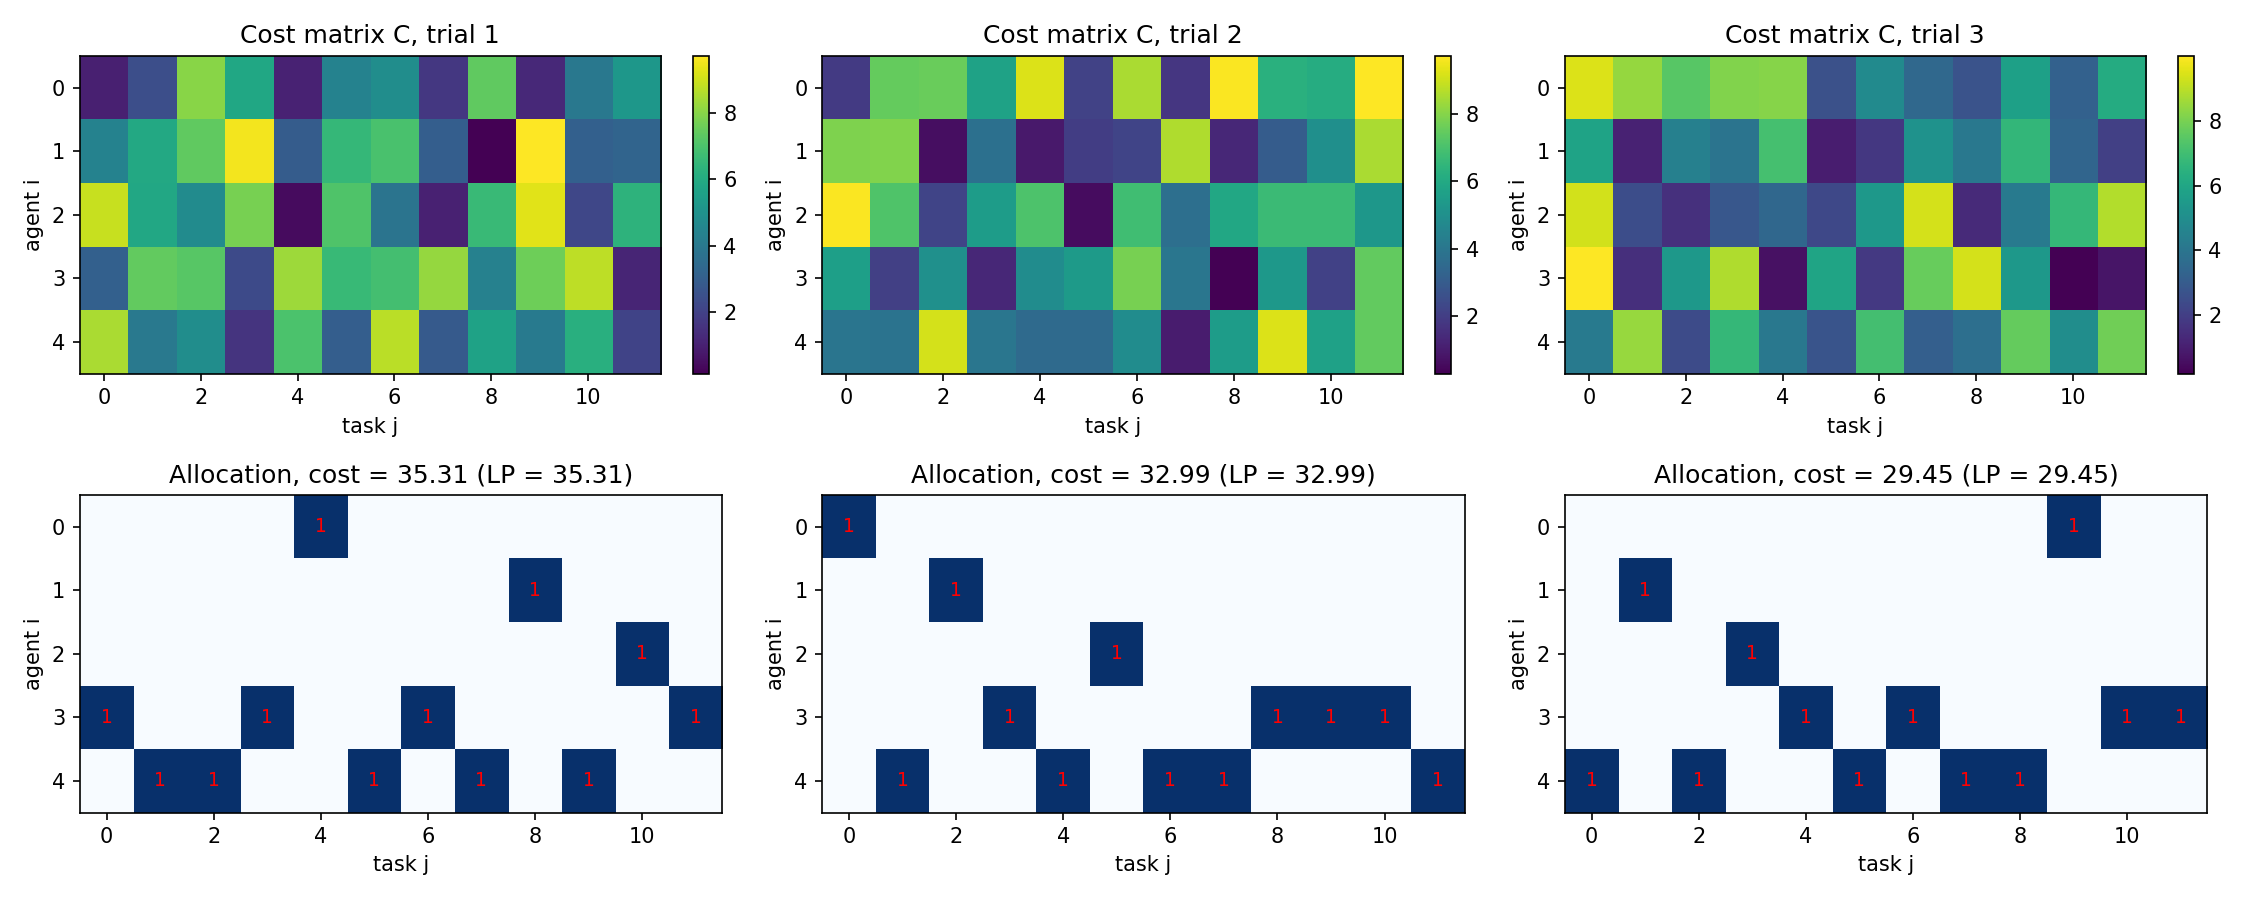
\includegraphics[width=\linewidth]{../p3_admm_task/allocations.png}
    \caption{Three trials with same $N, M, b, G$ and different cost matrices $C$. Top row: $C$. Bottom row: binary allocation.}
\end{figure}

\textbf{Observations.} Rounded ADMM cost equals the LP relaxation cost in all three trials ($35.310, 32.994, 29.452$). Agents $4$ and $5$ (large capacity) absorb most tasks, while agents $1, 2, 3$ (capacity $1$) each pick the single task where their row of $C$ is smallest relative to what the large-capacity agents can do. Which specific tasks land where depends entirely on $C$: the allocation shifts every time we resample $C$.

\lstinputlisting[caption={\texttt{problem3\_admm\_taskalloc.py}}]{../p3_admm_task/problem3_admm_taskalloc.py}

\end{solution}
\noindent\rule{7in}{2.8pt}

%%%%%%%%%%%%%%%%%%%%%%%%%%%%%%%%%%%%%%%%%%%%%%%%%%%%%%%%%%%%%%%%%%%%%%%%%
% Problem 4
%%%%%%%%%%%%%%%%%%%%%%%%%%%%%%%%%%%%%%%%%%%%%%%%%%%%%%%%%%%%%%%%%%%%%%%%%
\begin{problem}{4}
LASSO problem $\displaystyle \min_x \tfrac{1}{2}\|Ax - b\|_2^2 + \lambda \|x\|_1$. Write the ADMM iteration updates by giving the closed form solutions for $x$ and $z$ updates.
\end{problem}
\begin{solution}

\textbf{Variable splitting.} Introduce $z$ and rewrite as $\min f(x) + g(z)$ s.t. $x - z = 0$, with $f(x) = \tfrac{1}{2}\|Ax - b\|^2$ and $g(z) = \lambda\|z\|_1$.

\textbf{Scaled augmented Lagrangian} (with $u = y/\rho$):
\begin{align*}
    L_{\rho}(x, z, u) = \tfrac{1}{2}\|Ax - b\|^2 + \lambda\|z\|_1 + \tfrac{\rho}{2}\|x - z + u\|^2.
\end{align*}

\textbf{$x$-update (closed form).} Fix $z, u$. Setting the gradient to zero,
\begin{align*}
    A^{\top}(Ax - b) + \rho(x - z + u) = 0 \;\Longrightarrow\; (A^{\top}A + \rho I) x = A^{\top} b + \rho(z - u).
\end{align*}
Hence
\begin{align*}
    \boxed{\; x^{k+1} = (A^{\top}A + \rho I)^{-1} \big(A^{\top} b + \rho (z^k - u^k) \big). \;}
\end{align*}

\textbf{$z$-update (closed form).} Fix $x, u$. Completing the square,
\begin{align*}
    z^{k+1} = \arg\min_z \lambda\|z\|_1 + \tfrac{\rho}{2}\|z - (x^{k+1} + u^k)\|^2 = \mathrm{prox}_{(\lambda/\rho)\|\cdot\|_1}(x^{k+1} + u^k).
\end{align*}
The prox of the $\ell_1$ norm is soft thresholding $S_{\kappa}(v)_i = \mathrm{sign}(v_i)\max(|v_i| - \kappa, 0)$, so
\begin{align*}
    \boxed{\; z^{k+1} = S_{\lambda/\rho}\big(x^{k+1} + u^k\big). \;}
\end{align*}

\textbf{Dual update.}
\begin{align*}
    \boxed{\; u^{k+1} = u^k + (x^{k+1} - z^{k+1}). \;}
\end{align*}

\textbf{Numerical check.} With $m = 200$, $n = 500$, $A$ random Gaussian (columns unit norm), $x_{\mathrm{true}}$ sparse with $20$ non-zeros, $b = A x_{\mathrm{true}} + 0.01 \varepsilon$, $\lambda = 0.02 \|A^{\top} b\|_\infty$, $\rho = 1$: the algorithm converges in $72$ iterations, recovers $18/20$ true non-zeros with $3$ false positives, relative recovery error $\approx 0.051$.

\begin{figure}[H]
    \centering
    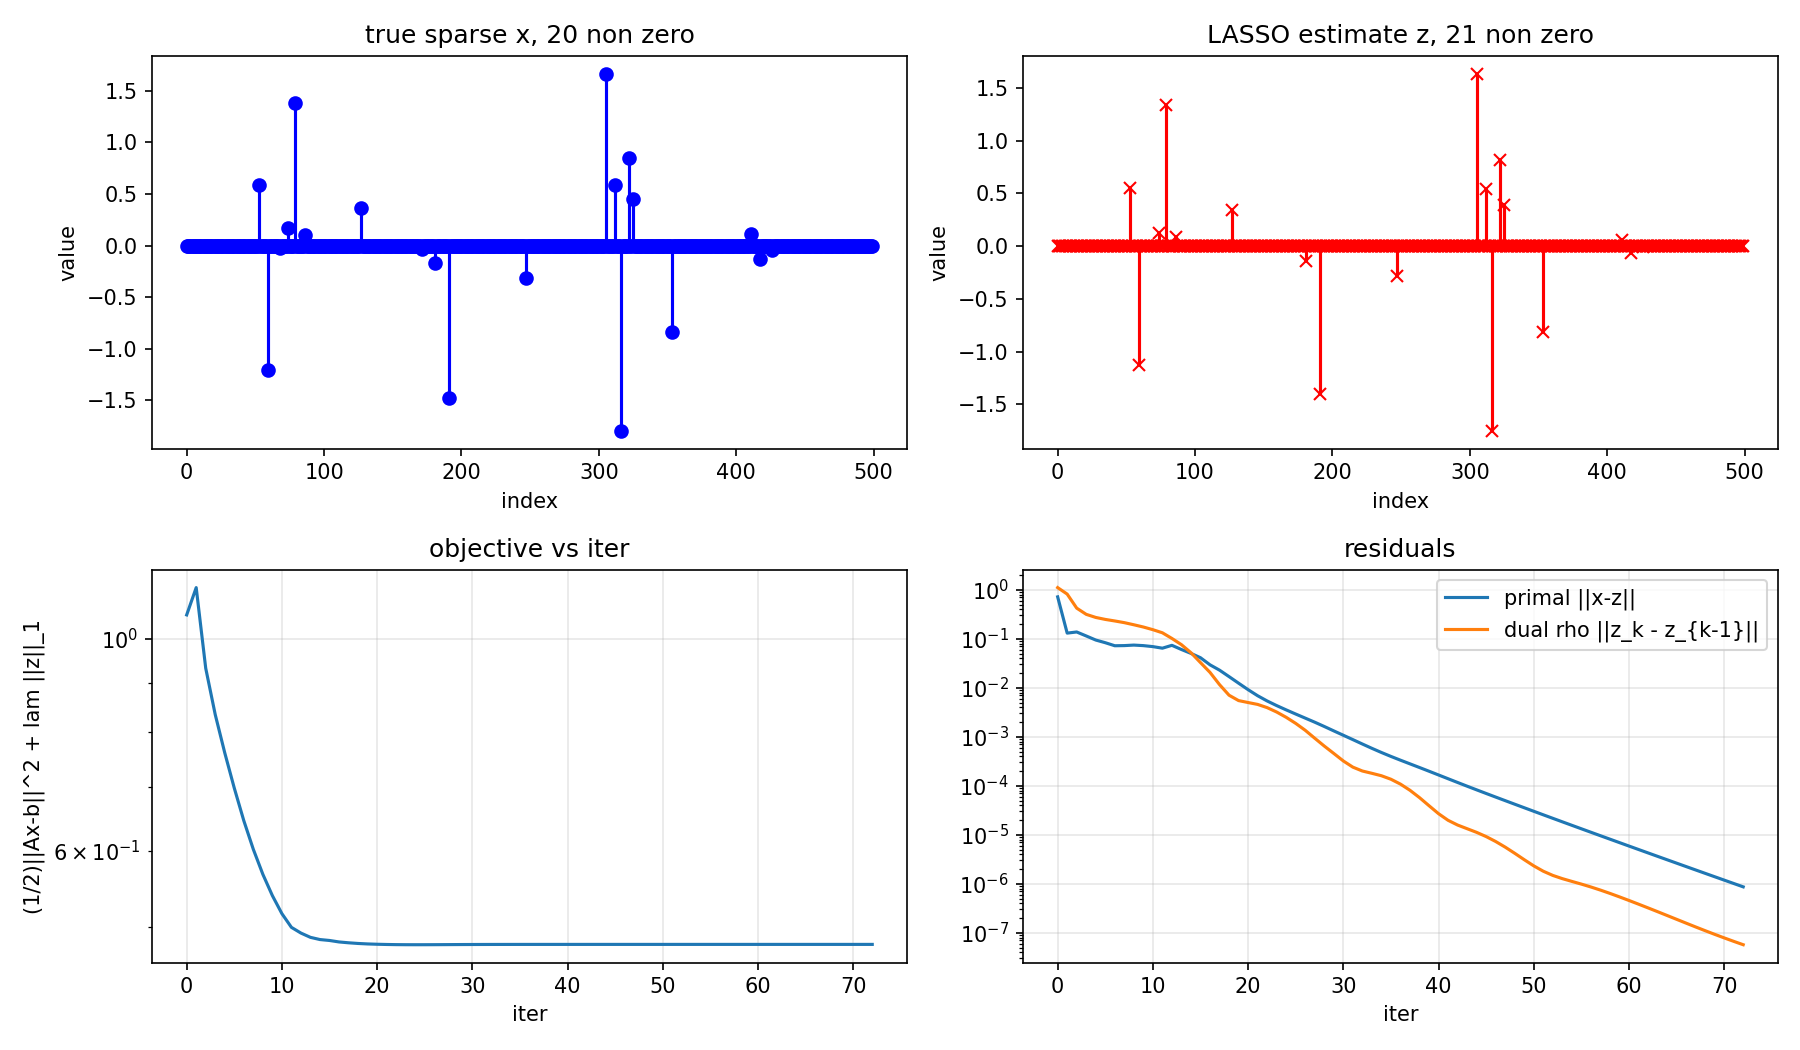
\includegraphics[width=\linewidth]{../p4_lasso/lasso.png}
    \caption{Top: true $x$ and recovered $z$. Bottom: objective and residuals.}
\end{figure}

\lstinputlisting[caption={\texttt{problem4\_lasso\_admm.py}}]{../p4_lasso/problem4_lasso_admm.py}

\end{solution}
\noindent\rule{7in}{2.8pt}

\end{document}
